
\section{System}

In this section, we introduce the main components of the system.
Our system is built with a pipeline style architecture giving it the advantage to run each section separately to allow stream processing without blocking the data flow of components (Figure~\ref{fig:system}).
The three logical components are divided into sections entitled \textit{Model} for entity resolution purposes,
\textit{Wikipedia Citation} to annotate cite-worthy documents,
and \textit{Slot Filling} to generate the actual slot values.


To discover facts for a single WP entity, the first step is to extract aliases of the entity.
%We use several approaches to get as many viable aliases as possible.
We extract several name variations from the Wikipedia.org API and from the WP entity page.
Also, if the entity type is \textit{person} we can change the order of user names to increase coverage (e.g. `Boris Berezovsky' $\rightarrow$ `Berezovsky, Boris').
Next, we iterate over documents in the stream and filter out all documents that do not explicitly contain a string matching 
the list of entities.
To extract relevant facts we perform pattern matching over each sentence that matches the entity based on a dictionary
of patterns.
If a sentence activates one of the patterns in the dictionary we emit this sentence as a candidate contribution
for the WP entity.
With the candidate set, we infer new facts from the set and clean up the set
by removing the set of values that violate a list of constraints such as duplicates.
%Lastly, we try to infer a new set of facts based on a list of rules.

%As a match is found from the content of the sentence to the patterns that we have generated regarding slot name, the associated slot value is extracted as a final result.

%\ceg{Discuss current system first. If you want to keep the decisions points that led to the current architecture, make it a subsection.}

\begin{figure}
\hspace{-10mm}
  \centering
%  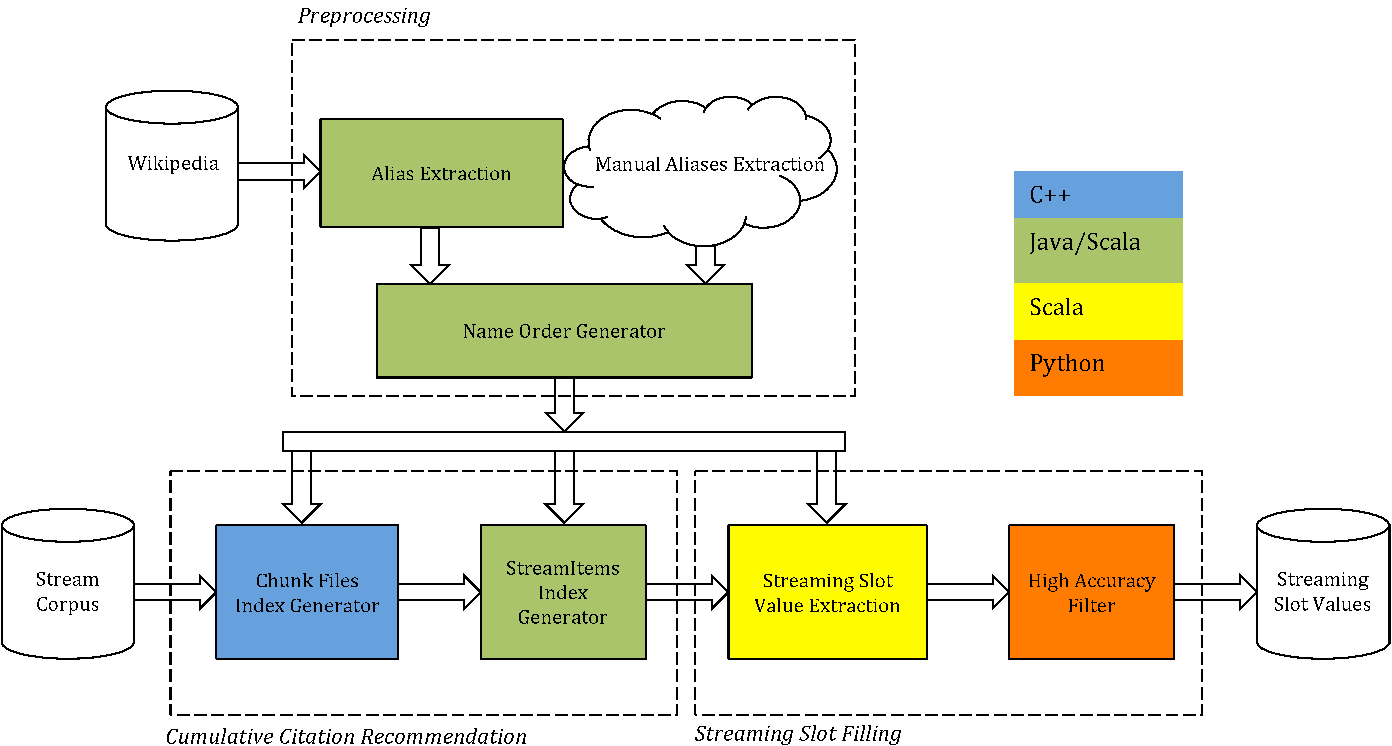
\includegraphics[width=6in]{./images/sdl-eps-converted-to.pdf}
  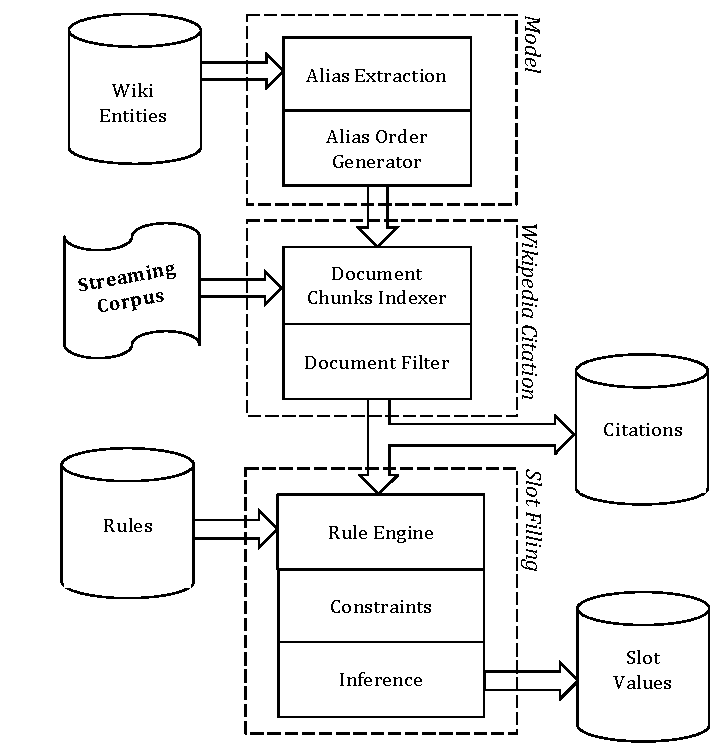
\includegraphics[width=8.5cm]{./images/System_Diagram_with_model_Vertical-crop.pdf}
% http://convert.neevia.com/pdfconvert/
  \vspace*{-.1in} 
  \caption{System Architecture.
  Components are logical groups noted with dotted boxes.}
  \label{fig:system}
  \vspace*{-.2in}
\end{figure}



\subsection{Entity Model}
\label{sec:entitymodel}

We use the Wikipedia.org API to retrieve aliases. 
The API allows us to requests pages that redirect users to an entity page.
For example, if a WP user tries to access the \textsl{William Henry Gates} entry they are sent to the page for 
\textsl{Bill Gates} --- we treat  such redirects as aliases. 
To extract more aliases we parse the HTML source of a WP entity page.
Using regular expressions we extract the bold phrases of the initial paragraph as aliases.
This method provides several inline aliases from the wiki page.
In WP page for the businesman `Boris Berezovski' , there is a mention of `Boris Abramovich Berezovsky' given in bold in the wiki page which obtained by regular expression extraction.

%\ceg{Do we know how many additional aliases this method provides?}.
%\ceg{Do you want to give a more concrete example of how this might now work? It may be TMI.}
%As an example of when this might not wirk, is that there might be occasions that some other topic is written in bold typesetting in the first paraph apart from the entity aliases itself but these are very rare.

We pass the full set of \textit{person} entities through rules for generating alternate name orders.
This module produces various forms of expressing entity names and titles.
For example, \textsl{Bill Gates} can be written as \textsl{Gates, Bill}.
This allows the system to capture various notation forms of aliases that appear in text documents.
%We refer to this part as \textit{Alias Order Generator}.

\subsection{Wikipedia Citation}
The goal of this section is to use the models created to discover a set of documents that are relevant to the WP entity.
%We perform exact string matching and treat all the documents that mention an entity equally likely to be citable.
As a stream of documents come in we first perform a string match between the model aliases and document text. 
We use this technique as a first filter with confidence because previous work states non-mentioning
documents have a low chance of being citable in Wikipedia \cite{JFrank12}.
Given our large number of aliases we can be confident that if an alias does not appear in a document it does not need to be cited.

Our system streams in documents in the form of chunk files.
Each chunk file contains thousands of documents.
This corpus of documents is processed by a two-layer filter system referred to as \textit{Document Chunk Filter} and \textit{Document Filter}.
The purpose of these filters is to reduce I/O cost while generating slot values for various entities.
Document Chunk Filter removes the chunk files that do not contain a mention of any of the desired entities.
Each chunk file may contain thousands of documents --- each document is expensive to process.
The Document Filter removes documents that do not contain a mention of an entity.
This two-level filter allows us to perform detailed slower processing over a smaller set of documents.
Not all chunk files contain mention of the entities so filtering out large chunk files early saves on I/O and processing.
Document Chunk Filter discards non-mentioning chunk files and promotes chunk files as soon as an entity mention is found.
%Processing StreamItems on the other hand is done in Java with ideas in mind for later on extensibility by adding other Java libraries.
The document filter additionally notes the sentences that contain entity mentions.
This data is passed to the Slot Filling system.


% Note: Describe the algorithms of each phase
% Talk in abstract terms not implementation.
% Use formal representations (Math, SQL etc)


%\ceg{This section should be structured as follows:
%1: Introduce CCR (Motivation, Expectations)
%2: Our high level approach
%3: Discussion of our design (Like already discussed)
%}


\subsection{Slot Filling}
\label{sec:slotfilling}
%\ceg{See the previous note.}
Streaming Slot Filling (SSF) extracts fact values from sentences according to a list of patterns.
Table~\ref{table:slotNameOntology} lists the slot relationships that we looks to extract.
In Figure~\ref{fig:system} we refer to this task as \textit{Slot Filling}. 

%Slot filling is done by pattern matching documents with manually produced patterns for slots of interest.
%The way we do this is by observing a sentence that has a mention of the entity or one of its coreference.
%An anchor word in the sentence related to the slot name is located and we match either left or right of
%the anchor word for potential slot values. 



%In the data set, we are given a date range of documents as training data. Instead of building a classifier we use pattern matching methods to find corresponding slot values for entities. 
%Pattern matching is simple to manipulate results and implement. Additionally, a classifier approach is more difficult to evaluate and explain results due to the lack of proper training data.

SSF reads documents filtered by the Wikipedia Citation step and fetches and tags sentences containing WP entities.
All entities are extracted from the document using a natural language processing
tool\footnote{Lingpipe (available in the dataset) provides entity tags
and in-document coreference. \url{http://alias-i.com/lingpipe/}}.
In the next section, we describe how WP entities are matched against the set of patterns.
Following, we discuss out approach to inference over the extracted facts.

\begin{algorithm}
  \caption{Slot Value Extraction Pseudocode}
  \textbf{List of entities $\mathcal{E} = \{e_0, \ldots, e_{170}\}$}\\
  \textbf{List of patterns $P = \{p_0, \ldots, p_{|P|}\}$}\\
  \textbf{List of documents containing entities $\mathcal{S} = \{s_0, \ldots, s_{|\mathcal{S}|}\}$}\\

  \begin{algorithmic}%[1]
    \FOR{$si \in \mathcal{S}$}
    \FOR{$sentence \in si$}
    \FOR{$entity \in \mathcal{E}$}
    \IF{Contains($sentence$, $entity$)}
    \FOR{$pattern \in P $ suitable for $entity$} 
    \IF{Satisfies($sentence$, $pattern$)}
    \STATE Emit($sentence$, $pattern$)
  \ENDIF
\ENDFOR
          \ENDIF
        \ENDFOR
      \ENDFOR
    \ENDFOR
  \end{algorithmic}
\end{algorithm}


\subsubsection{Rule Engine}

%\textbf{Format of Patterns.}
A pattern is a template of a fact to be extracted and added to a WP entity.
Patterns are used to find and extract facts from text.
A pattern $\mathcal{P}$ is represented as a five-tuple $\mathcal{P} = \langle p_1, p_2, p_3, p_4, p_5 \rangle$.


The first value, $p_1$ represents the type of entity.
These entity types are in the set $\{\text{\tt FAC}, \text{\tt ORG}, \text{\tt PER} \}$ where \texttt{FAC} represents a type of facility, \texttt{ORG} represents an organization and \texttt{PER} represents a person.
%\texttt{FAC}, \texttt{ORG} and \texttt{PER} are Lingpipe entity types.
 $p_2$ represents a slot name.
A list of slot names is present in Table~\ref{table:slotNameOntology}.
The third element $p_3$ is the pattern content --- 
a string found in the sentence that identifies a slot name.
The extractor looks specifically for pattern content.
The pattern evaluator uses a direction (\texttt{left} or \texttt{right}) found in $p_4$ to explore sentence.
The final element $p_5$ represents the slot value of a pattern. 
%When we match one pattern, we match all the 
%fields except the third field, which is extracted as the final result.
The type of slot value may be the entity type labeled by the named entity extractor,
a noun phrase (\texttt{NP}) tagged by a part of speech tagger\footnote{OpenNLP was used for part of speech tagging. \url{http://opennlp.apache.org/}} or a phrase described in the pattern list.
%For these three kinds of patterns, we implement them in different ways accordingly. 

%Next, we explain the patterns with more details, an example of which can be found in Figure~\ref{fig:pattern}. 
Figure~\ref{fig:pattern} contains the example sentence from the introduction labeled by the rule engine. The matching pattern is $\langle$\texttt{PER, DateOfDeath, \textit{passed away}, right, NP}$\rangle$. In the figure, `Boris Berezovsky' matches as an alias for WP entity \textsl{wiki/Boris\_Berezovsky\_(businessman)}, DateOfDeath is the slot name, `passed away' is the content of the pattern, direction is `Right' and the actual value of the slot is `March 2013' which is a Noun Phrase.

%\textbf{Types of patterns}
There are three types of patterns, each distinguished by different types of slot values ($p_5$) in the patterns.
The matching methods using these three types of patterns are implemented according to the different structures of slot values.

\begin{figure}
\centering
%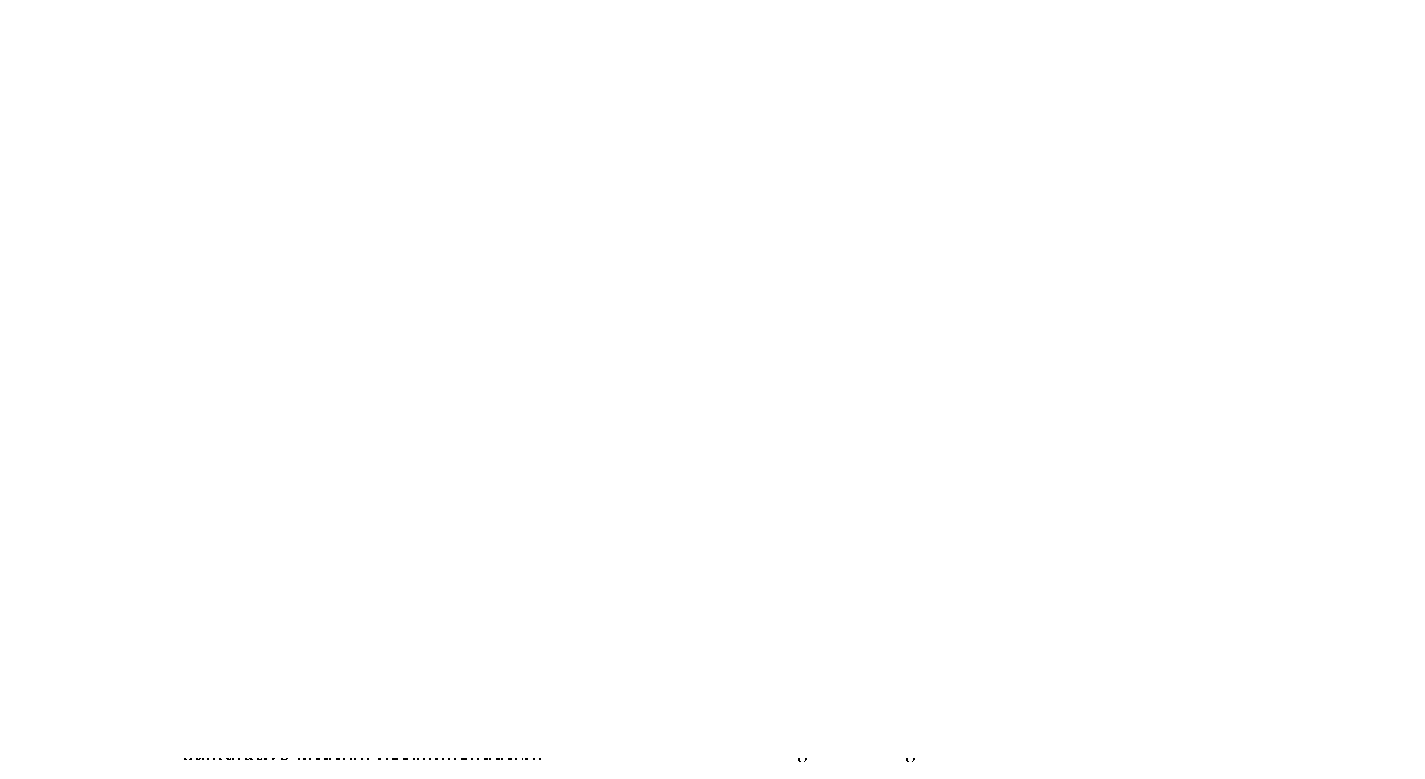
\includegraphics[width=4.5in]{./images/system.eps}
%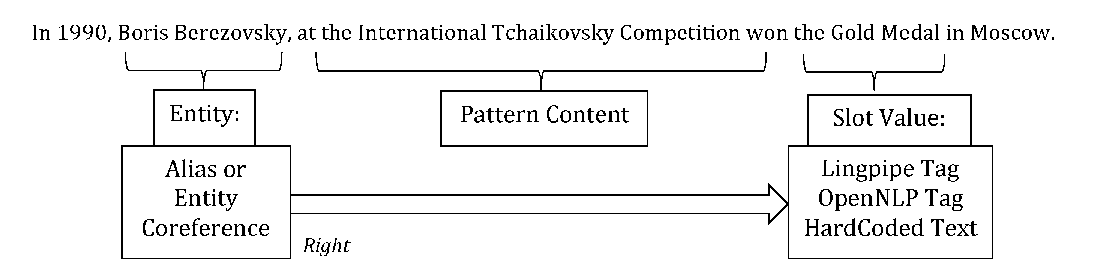
\includegraphics[width=6in]{./images/Pattern.eps}
%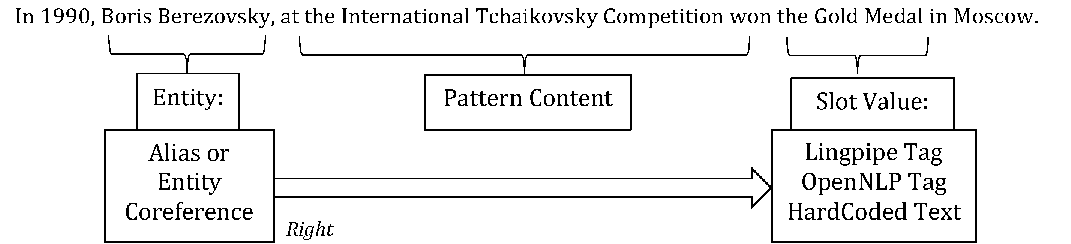
\includegraphics[width=6in]{./images/Pattern-eps-converted-to.pdf}
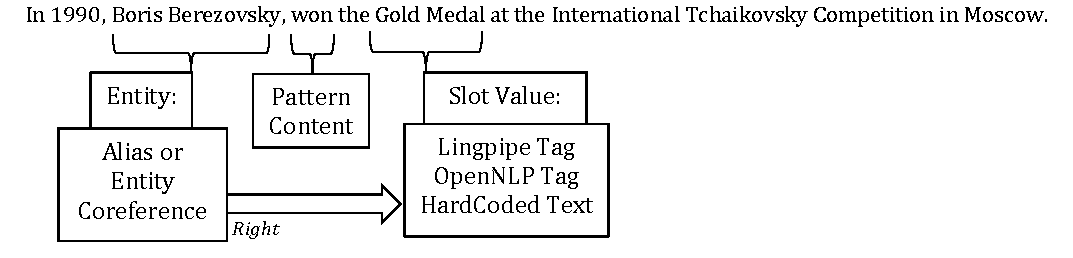
\includegraphics[width = 11cm]{./images/Pattern-crop.pdf}
% cropped pdf created using $ pdfcrop Pattern.pdf
\vspace*{-.1in}
\caption{Pattern matching for rule evaluation. The slot value is on the right side of the 
entity. The pattern context discovered is `passed away' with a value of `March 2013'. This conforms to type II of our pattern categories.}\label{fig:pattern}
\vspace*{-.2in}
\end{figure}
 
\textbf{Type I.} This pattern type is driven by the entity type.
For example, in pattern $\langle$\texttt{PER, FounderOf, \textit{founder}, right, ORG}$\rangle$ the \texttt{PER} 
tag means the entity we are finding slot values for is a PER entity;
\texttt{FounderOf} means this is a pattern for FounderOf slot.
\textit{founder} is the word we match in a sentence - the content of pattern occuring in the sentence;
\texttt{right} means that we are going to the right part of the sentence to match the pattern and find the slot value;
ORG means the slot value should be a ORG entity to the right of the entity.

\textbf{Type II.} This pattern type, after finding a matching pattern content, looks for a noun phrase (NP)
that is representative of the slot value.
For example, pattern $\langle$\texttt{PER, AwardsWon, \textit{awarded}, right, NP}$\rangle$
is looking for a noun phrase after the \textit{awarded} that may represent an award.
Titles and awards are not named entity tagged hence the use of the part of speech tagger to fetch the noun phrases.

\textbf{Type III.} These types of facts are best discovered by hard coding the slot values.
Examples of these include time phrases: $\langle$\texttt{PER, DateOfDeath, \textit{died}, right, \textit{last night}}$\rangle$.
In this pattern, the phrase \textit{last night} is exactly searched in the text {last night} to the right of the term \textit{died}.
The intuition behind this pattern is in news articles that report events in the past relative to the article. 
For example, an article will mention that  
a person died `last night' instead of mentioning precise date-time information.
Additionally, part of speech taggers and name entity extractors did not label these terms such as 
\textit{last night} as a DATE entity. 


\subsection{Constraints and Inference}%\ceg{what specifically about the algorithm causes duplicates and errors? --- I asked Yang to elaborate on this as he is more familiar but still not sure what's causing those issues} 
\label{sec:constraintsandinference}

Our data set contains some duplicate webpages, webpage texts with similar content, 
and some of the entity tags are incomplete.
This causes some duplicates or highly similar content in the extracted list. 
We implement a filter to remove duplicates or the fact extractions that match patterns that are general and highly susceptible to be noisy.
The data contains duplicates and incorrect extractions.
We define rules to read ordered sets of facts to sanitize the output.
The input is processed in time order, in a tuple-at-a-time fashion to allow rules to discover noisy slots 
that appears in close proximity.
%We found that the proximity of an extraction has a high correlation on the presence of duplicates. 
We define two classes of rules: \textit{deduplication} and \textit{inference} rules.

The output contains many duplicate entries.
As we read the list of extracted slots we create rules to define ``duplicate''.
Duplicates can be present in a window of rows; we use a window size of 2 meaning we only be adjacent rows.
Two rows are duplicates if they have the same exact extraction or if the rows have the same slot name and a similar slot value or if the extracted sentence for a particular slot types come from the same sentence.

New slots can be deduced from existing slots by defining inference rules.
For example, two slots for the task are ``FounderOf'' and ``FoundedBy''.
A safe assumption is these slot names are biconditional logical connectives with the entities and slot values.
Therefore, we can express a rule ``$X$ FounderOf $Y$'' $\leftrightarrow$ ``$Y$ FoundedBy $X$'' where $X$ and $Y$ are single unique entities.
Additionally, we found that the slot names ``Contact\_Meet\_PlaceTime'' could be inferred as ``Contact\_Meet\_Entity'' if the Entity was a FAC and the extracted sentence contained an additional ORG/FAC tag.
We also remove erroneous slots that have extractions that are thousands of characters in length or tool small.
Errors of extracting long sentences can typically be attributed to poor sentence parsing of web documents.
We have some valid ``small'' extractions. For example, a comma may separate a name and a title (e.g. ``John, Professor at MIT'').
But such extraction rules can be particularly noisy, so we check to see if the extracted values have good entity values.
